%%%%%%%%%%%%%%%%%%%%%%%%%%%%%%%%%%%%%%%%%
% Journal Article
% LaTeX Template
% Version 1.4 (15/5/16)
%
% This template has been downloaded from:
% http://www.LaTeXTemplates.com
%
% Original author:
% Frits Wenneker (http://www.howtotex.com) with extensive modifications by
% Vel (vel@LaTeXTemplates.com)
%
% License:
% CC BY-NC-SA 3.0 (http://creativecommons.org/licenses/by-nc-sa/3.0/)
%
%%%%%%%%%%%%%%%%%%%%%%%%%%%%%%%%%%%%%%%%%

%----------------------------------------------------------------------------------------
%	PACKAGES AND OTHER DOCUMENT CONFIGURATIONS
%----------------------------------------------------------------------------------------

\documentclass[twoside,onecolumn]{article}

\usepackage{blindtext} % Package to generate dummy text throughout this template 
\usepackage{graphicx}
\graphicspath{ {Imagenes/} }
\usepackage[sc]{mathpazo} % Use the Palatino font
\usepackage[T1]{fontenc} % Use 8-bit encoding that has 256 glyphs
\linespread{1.05} % Line spacing - Palatino needs more space between lines
\usepackage{microtype} % Slightly tweak font spacing for aesthetics

\usepackage[english]{babel} % Language hyphenation and typographical rules

\usepackage[hmarginratio=1:1,top=32mm,columnsep=20pt]{geometry} % Document margins
\usepackage[hang, small,labelfont=bf,up,textfont=it,up]{caption} % Custom captions under/above floats in tables or figures
\usepackage{booktabs} % Horizontal rules in tables

\usepackage{lettrine} % The lettrine is the first enlarged letter at the beginning of the text

\usepackage{enumitem} % Customized lists
\setlist[itemize]{noitemsep} % Make itemize lists more compact

\usepackage{abstract} % Allows abstract customization
\renewcommand{\abstractnamefont}{\normalfont\bfseries} % Set the "Resumen" text to bold
\renewcommand{\abstracttextfont}{\normalfont\small\itshape} % Set the abstract itself to small italic text

\usepackage{titlesec} % Allows customization of titles
\renewcommand\thesection{\Roman{section}} % Roman numerals for the sections
\renewcommand\thesubsection{\roman{subsection}} % roman numerals for subsections
\titleformat{\section}[block]{\large\scshape\centering}{\thesection.}{1em}{} % Change the look of the section titles
\titleformat{\subsection}[block]{\large}{\thesubsection.}{0.2em}{} % Change the look of the section titles

\usepackage{fancyhdr} % Headers and footers
\pagestyle{fancy} % All pages have headers and footers
\fancyhead{} % Blank out the default header
\fancyfoot{} % Blank out the default footer
\fancyhead[C]{Comparación de despliegue de un gestor de base de datos NoSQL mediante Docke $\bullet$ Junio 2019 $\bullet$ Trabajo Final} % Custom header text
\fancyfoot[RO,LE]{\thepage} % Custom footer text

\usepackage{titling} % Customizing the title section

\usepackage{hyperref} % For hyperlinks in the PDF

%----------------------------------------------------------------------------------------
%	TITLE SECTION
%----------------------------------------------------------------------------------------
\setlength{\droptitle}{-4\baselineskip} % Move the title up

\pretitle{\begin{center}\Huge\bfseries} % Article title formatting
\posttitle{\end{center}} % Article title closing formatting
\title{Comparación de Despliegue de un Gestor de Base de Datos NoSQL Mediante Docker} % Article title
\author{%
\textsc{Marko Antonio Rivas Rios} \\[1ex] % Your name
\textsc{Jorge Luis Mamani Maquera} \\[1.01ex] % Your name
\textsc{Orlando Antonio Acosta Ortiz} \\[1.02ex] % Your name
\textsc{Yofer Nain Catari Cabrera} \\[1.03ex] % Your name
\textsc{Orestes Ramirez Ticona} \\[1.04ex] % Your name
\textsc{Roberto Zegarra Reyes} \\[1.05ex] % Your name
\normalsize Universidad Privada de Tacna \\  % Your institution
\normalsize {} % Your email address
%\and % Uncomment if 2 authors are required, duplicate these 4 lines if more
%\textsc{Jane Smith}\thanks{Corresponding author} \\[1ex] % Second author's name
%\normalsize University of Utah \\ % Second author's institution
%\normalsize \href{mailto:jane@smith.com}{jane@smith.com} % Second author's email address
}
\date{Junio 22, 2019} % Leave empty to omit a date
\renewcommand{\maketitlehookd}{%
\begin{abstract}
\begin{center}
\textbf{Resumen}
\end{center}
\noindent Docker es un proyecto open source creado en 2013 y que ha supuesto una revolución para el desarrollo y despliegue de operaciones. Docker abstrae el hardware y el sistema operativo del host ejecutando las aplicaciones en contenedores, compartimentos aislados que contienen todos los recursos para una aplicación o servicio. En este trabajo veremos cómo usar Docker para el desarrollo de aplicaciones sencillas, aprendiendo a desplegar una base de datos NOSQL con Docker.
\begin{center}
\textbf{Abstract}
\end{center}
\noindent Docker is an open source project created in 2013 and which has been a revolution for the development and deployment of operations. Docker abstracts the host's hardware and operating system by running the applications in containers, isolated compartments that contain all the resources for an application or service.
In this work we will see how to use Docker for the development of simple applications, learning how to deploy a NOSQL database with Docker.
\end{abstract}
}


%----------------------------------------------------------------------------------------

\begin{document}

% Print the title
\maketitle

%----------------------------------------------------------------------------------------
%	ARTICLE CONTENTS
%----------------------------------------------------------------------------------------

\section{Introducción}

\lettrine[nindent=0em,lines=2]{E}l potente concepto de Microservicios está cambiando poco a poco la industria. Grandes servicios monolíticos están dando paso lentamente al enjambre microservicios pequeños y autónomos que trabajan en conjunto. El proceso va acompañado de otra tendencia del mercado: la contenerización. Juntos, ayudan a construir sistemas  sin precedentes. La contenerización cambia no sólo la arquitectura de los servicios, sino también la estructura de ambientes utilizados para crearlos.
\textbf{}\\
Ahora, cuando el software se distribuye en contenedores, los desarrolladores tienen plena libertad para decidir qué aplicaciones necesitan. Como resultado, incluso los entornos complejos, como los servidores de grades bases de datos e infraestructura de análisis complejos pueden crear instancias en cuestión de segundos. El desarrollo de software se hace más fácil y más eficaz.

\section{Materiales y Métodos}
\subsection{Materiales}
	\begin{itemize}
		\item Virtualización activada en el BIOS
		\item Docker Desktop
		\item Windows 10 64bit: Pro, Enterprise o Education, con al menos 4GB de RAM.
	\end{itemize}
\subsection{Métodos}
	\begin{itemize}
		\item Se utilizo como material artículos y libros relacionados a la base de datos NoSQL y sus tipos, así como páginas web.
	\end{itemize}
\begin{flushright}
\begin{itemize}
%------------------------------------------------

\section{Marco Teórico}

\textbf{}\\
\subsection{Creación de una base de datos NoSQL en docker}
\textbf{}\\


\textbf{}\\
\subsection{Inserción de datos y Consulta de datos (en una base de datos NOSQL)}
\begin{center}
		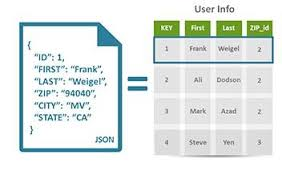
\includegraphics[width=9cm]{./Imagenes/6}
		\end{center}	
\textbf{}\\
Existen varias diferencias con respecto a cómo los distintos tipos de bases de datos permiten a los usuarios / aplicaciones realizar consultas. Desde las consultas más básicas por clave primaria, como por ejemplo, los almacenes clave – valor, pasando por otros que ofrecen un acceso a la información algo más complejo. En este terreno se encontrarían las bases de datos documentales.
\begin{center}
		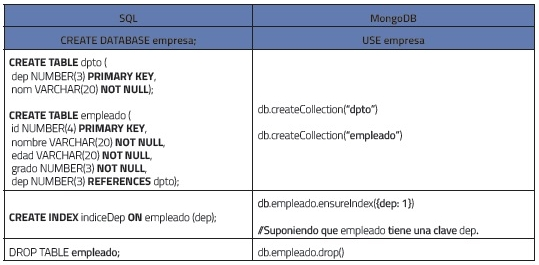
\includegraphics[width=9cm]{./Imagenes/1}
		\end{center}	
\textbf{}\\
En general, la flexibilidad y la riqueza de las querys no son demasiado elevadas, puesto que lo que se prima por encima de las consultas es el rendimiento y la escalabilidad, por lo que es habitual que se delegue a la aplicación el implementar opciones más avanzadas en este terreno.
\textbf{}\\
Un método de consulta llamado Companion SQL database consiste en tener una base de datos auxiliar (que puede ser una base de datos SQL o una TextDB) de forma que se utilice esta secundaria para almacenar ciertos metadatos importantes para realizar la búsqueda, y se empleen para facilitar la búsqueda posterior en el contenedor NoSQL.
\begin{center}
		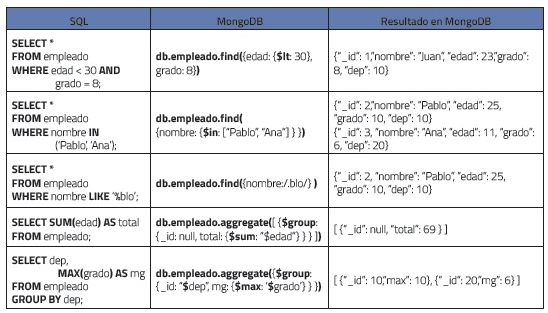
\includegraphics[width=9cm]{./Imagenes/2}
		\end{center}	
\textbf{}\\
Búsqueda local dispersa. Otra forma de realizar consultas consiste en, puesto que se tiene el conjunto de datos repartido entre los distintos servidores, repartir de igual modo la consulta, de forma que cada servidor ejecute localmente cada consulta y reenvíe los
resultados a un nodo maestro, que sería el encargado de juntar todos los resultados y presentárselos a la aplicación.
\textbf{}\\
Arboles B+ Distribuidos.
\textbf{}\\
Una forma eficiente de acelerar las búsquedas consiste en mantener un árbol B+ que forme un índice de entradas a la base de datos NoSQL (Aquilera, Golab and Shah 2008).
\textbf{}\\
El procedimiento consistiría en sacar los valores hash de los atributos que nos interese indexar, y construir con ellos el árbol B+. Cuando se quiera realizar una consulta, se comenzará desde la raíz y se irá descendiendo en orden hasta llegar a la hoja correspondiente, que nos dará la entrada concreta donde se encuentra el registro que se está buscando.
\begin{center}
		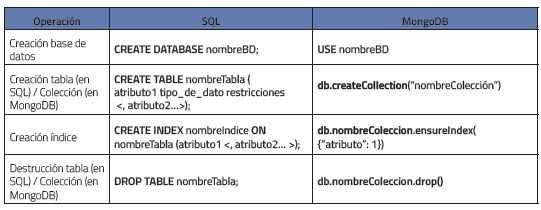
\includegraphics[width=9cm]{./Imagenes/3}
		\end{center}	
\textbf{}\\
Al tratarse de un árbol B+, se debe tener en cuenta las particularidades de este tipo de estructura de datos a la hora de realizar los mantenimientos necesarios, las inserciones y borrados que puedan hacer redimensiones en el árbol, etc.


\textbf{}\\
\subsection{Comparacion de distintos tipos de base de datos NoSQL}
\textbf{}\\Dependiendo de la forma en la que almacenen la información, nos podemos encontrar varios tipos
distintos de bases de datos NoSQL. Veamos los tipos más utilizados.
 \begin{itemize}
		\item Bases de datos clave – valor
                     \item Bases de datos documentales
		\item Bases de datos en grafo
		\item Bases de datos orientadas a objetos
	           \end{itemize}
\begin{center}
		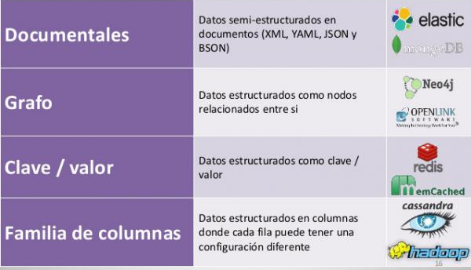
\includegraphics[width=9cm]{./Imagenes/7}
		\end{center}	
\textbf{}\\


\textbf{CouchDB: }\\ CouchDB es catalogado muchas veces como una base de datos NoSQL, un término que se hizo cada vez más popular a finales de 2009 y principios de 2010. Si bien este término es una caracterización más bien genérica de una base de datos, o almacén de datos, sí define claramente un descanso de SQL tradicional bases de datos. Una base de datos CouchDB carece de un esquema o estructuras de datos pre-definidos rígidos tales como tablas. \textbf{}\\
Los datos almacenados en CouchDB es un documento (s) JSON. La estructura de los datos, o documento(s), puede cambiar dinámicamente para adaptarse a las necesidades cambiantes. 
CouchDB es una base de datos que abarca por completo la web. Almacene sus datos con documentos JSON. Tenga acceso a sus documentos y consultar sus índices con su navegador web, a través de HTTP.Índice, combinar y transformar sus documentos con JavaScript. CouchDB funciona bien con la web moderna y aplicaciones móviles. Usted puede incluso servir aplicaciones web directamente de CouchDB. Y usted puede distribuir sus datos o sus aplicaciones, de manera eficiente mediante la replicación incremental de los CouchDB. CouchDB soporta configuraciones maestro-maestro con detección automática de conflictos. \textbf{}\\
CouchDB viene con una serie de características, como la transformación de documentos sobre la marcha y notificaciones de cambio en tiempo real, que hace que el desarrollo de aplicaciones web una brisa. Incluso viene con un fácil utilizar la consola de administración web.\textbf{}\\
\textbf{}\\
 \textbf{Las principales características son las siguientes:}\\
\textbf{}\\
\textbf{•	Almacenamiento de documentos:}\\ Almacena los datos como documentos esto es, uno o más pares campo/valor expresados en JSON. Los valores de los campos pueden ser datos simples como cadenas de caracteres, números o fechas. Pero también se pueden usar listas ordenadas y vectores asociativos. Todos los documentos en una base de datos CouchDB tienen un identificador único y no requieren un esquema determinado.
\textbf{}\\
\textbf{}\\
\textbf{•	Vistas e índices Map/Reduce:}\\
 Los datos almacenados se estructuran por medio de vistas. En CouchDB, cada vista se construye por medio de una función JavaScript que actúa como la mitad Map de una operación map/reduce. La función recibe un documento y lo transforma en un único valor, retornándolo. CouchDB puede indexar vistas y mantener actualizados esos índices a medida que se agregan, eliminan o actualizan documentos.
\textbf{}\\
\textbf{•	Arquitectura distribuida con replicación: }\\
Se diseñó con teniendo en mente la replicación bidireccional (o sincronización) y la operación off-line. Eso significa que múltiples réplicas pueden tener cada una sus propias copias de los mismos datos, modificarlas y luego sincronizar esos cambios en un momento posterior.
\textbf{}\\
\textbf{}\\
\textbf{•	Interfaz REST:}\\
 Todos los ítems tienen una URI única que queda expuesta vía HTTP. REST usa los métodos HTTP POST, GET, PUT y DELETE para las cuatro operaciones básicas CRUD (Create, Read, Update, Delete) con todos los recursos.
\textbf{}\\
\textbf{}\\
\textbf{•	Consistencia Eventual:}\\
 Garantiza consistencia eventual para poder ofrecer tanto disponibilidad como tolerancia a las particiones.
\textbf{}\\
\textbf{}\\
\textbf{•	Hecha para operar offline:}\\
 Puede replicar datos a dispositivos (como smartphones) que pueden quedar offline y manejar automáticamente la sincronización de los datos cuando el dispositivo vuelve a estar en línea.


\textbf{}\\
\textbf{}\\
\textbf{}\\
\textbf{}\\

\textbf{Neo4j:}\\
 Es una base de datos orientada a grafos escrita en Java, es decir la información se almacena de forma relacionada formando un grafo dirigido entre los nodos y las relaciones entre ellos. Se integra perfectamente con múltiples lenguajes como Java, PHP, Ruby, .Net,  Python, Node, Scala, etc. La base de datos está embebida en un servidor Jetty. Está especialmente indicada para modelar redes sociales y sistemas de recomendación.\textbf{}\\
Se distribuye en dos versiones: la community edition (open source) y la Enterprise edition. Para hacer pruebas de concepto nos basta con la community edition pero si quieres sacarle todo el partido a Neo4j la opción enterprise es la más recomendable ya que permite ponerla en cluster, monitorización, backups en caliente y un sistema de cache de alto rendimiento, además de soporte de sus creadores.\textbf{}\\
Otra de las ventajas que tiene Neo4j es que se pueden efectuar las consultas directamente a través de un API Rest lo que hace especialmente interesante su integración con aplicaciones web.
\textbf{}\\
\textbf{Principales características de neo4j:}\\
\textbf{}\\
•	Alto desempeño y alta disponibilidad (Escalamiento de lectura) Soporte sólido y real para transacciones ACID.
\textbf{}\\
•	Escalable: 32 miles de millones de Nodos, 32 miles de millones de Relaciones, 64 miles de millones de Propiedades.
\textbf{}\\
•	Servidor con una API REST o usable como una biblioteca Java.


\textbf{}\\
\textbf{}\\
\textbf{}\\
\section{Resultados}
\textbf{Comparaciones de 2 Bases de Datos NoSQL}\\
\subsection{Grafos}


\textbf{}\\
\textbf{}\\
\textbf{}\\
\textbf{}\\



\subsection{ Tabular (Column-Store)}

\textbf{}\\
\textbf{}\\
\textbf{}\\
\textbf{}\\



\subsection{Documental}
\textbf{}\\
\textbf{}\\
\textbf{}\\
\textbf{}\\




\subsection{Clave-Valor }
\textbf{}\\
\textbf{}\\
\textbf{}\\
\textbf{}\\






\section{Discusión}
\textbf{}\\
\textbf{}\\
\textbf{}\\
\textbf{}\\




\section{Conclusiones}
\textbf{}\\
\textbf{}\\
\textbf{}\\
\textbf{}\\




\textbf{}\\
\textbf{}\\
%----------------------------------------------------------------------------------------
%	REFERENCE LIST
%----------------------------------------------------------------------------------------

\begin{thebibliography}{99} % Bibliography - this is intentionally simple in this template



\newblock 
1. http://revistatelematica.cujae.edu.cu/
index.php/tele/article/view/23/21
 \break
\newblock 
2. https://programarfacil.com/blog/
que-es-un-orm/
\break
\newblock 
3. https://www.beeva.com/beeva-view/tecnologia/mas-alla-de-la-virtualizacion-contenedores/
\break
\newblock
4. https://searchdatacenter.techtarget.com/
es/definicion/virtualizacion-basada-en-contenedores-virtualizacion-a-nivel-de-sistema-operativo
\break
\newblock
5. https://www.incibe-cert.es/blog/asegurando-virtualizacion-tus-sistemas-control
\break
\newblock
6. http://www.datakeeper.es/?p=716
\break
\newblock
7.https://sigmodrecord.org/publications/sigmodRecord/1012/pdfs/04.surveys.cattell.pdf
\break
\newblock
8.https://ieeexplore.ieee.org/abstract/document/6625441
\break
\newblock
9.-http://nosql-database.org/
\break
\newblock {\em }
 
\end{thebibliography}



%----------------------------------------------------------------------------------------
\end{itemize}
\end{flushright}
\end{document}

